\documentclass[11pt]{article}
\usepackage[margin= 1in]{geometry}
\usepackage{mathptmx}
\usepackage[scaled = 1]{helvet}
\usepackage{courier}
\usepackage{lipsum}% just to generate filler text
\usepackage{setspace}
\usepackage{soul}
\doublespacing
\usepackage[utf8]{inputenc}
\usepackage{natbib}
\usepackage{graphicx}
\usepackage{amsmath}
\usepackage{amssymb}
\usepackage{mathrsfs} 
\usepackage{subcaption}
\usepackage{hyperref}
\usepackage{lipsum}
\usepackage{booktabs}
\usepackage[nomarkers]{endfloat}
\usepackage{capt-of}
\renewcommand{\efloatseparator}{\vfill}
% \usepackage[utf8]{inputenc}
\usepackage{authblk}
% \usepackage{setspace}
% \usepackage[margin=1.25in]{geometry}


\title{REGENS: an open source Python package for generating synthetic whole genomes}
% \renewcommand\maketitlehookc{\vspace{-25ex}}
\date{}

%%%%%% Authors %%%%%%
\author[1]{John T. Gregg}
\author[1]{Trang T. Le}
\author[1]{Jason H. Moore}

%%%%%% Affiliations %%%%%%
\affil[1]{Department of Biostatistics, Epidemiology and Informatics, University of Pennsylvania, Philadelphia, PA 19087, USA.}
\affil[*]{Corresponding author. Email: jhmoore@upenn.edu}

\begin{document}
\maketitle

\begin{singlespace}
\section{Summary}

REcombinatory Genome ENumeration of Subpopulations (REGENS) is an open source Python package that simulates autosomal genotypes by concatenating real individuals' genomic segments in a way that preserves their linkage disequilibrium (LD), which is defined as statistical associations between alleles at different loci \cite{slatkin2008linkage}. Recombining segments in a way that preserves LD simulates autosomes that closely resemble those of the realistic input population \cite{source:1} because real autosomal genotypes can be accurately modeled as genomic segments from a finite pool of heritable association structures (LD haplotypes) \cite{source:3}.
REGENS can also simulate mono-allelic and epistatic single nucleotide variant (SNV) effects of any order without perturbing the simulated LD pattern.
The SNVs involved in an effect can contribute additively, dominantly, recessively, only if heterozygous, or only if homozygous.
All simulated effects contribute to the value of either a binary or continuous biological trait (phenotype) with a specified mean value and a specified amount of random noise.  

\section{Statement of need}

The goal of most genome-wide association studies (GWAS) is to identify associations between single nucleotide variants (SNVs) and a phenotype to inform researchers and clinicians about potentially causative genetic factors. Completing this task will require overcoming numerous challenges such as insufficient sample sizes and over-representation of European ancestries \cite{torkamani2018personal}. Computational biologists build machine learning models that look for genetic associations in such unconventional datasets, but the majority of genetic associations have yet to be discovered \cite{source:4}. Researchers can use simulated datasets with known ground truths to assess the effectiveness of an algorithm, such as the power to detect epistatic effects with dimensionality reduction techniques \cite{source:11}. The more closely simulated data matches real-world data, the more accurate such test results will be. Since humans of different ancestry have different LD patterns \cite{source:5}, a simulation that can replicate those patterns from a small number of real samples is desirable. Therefore, intended users of REGENS are computational biologists who aim to test a statistical learning model on simulated GWAS data with precise realistic LD patterns.\\

\section{Algorithm overview}
Two genomic segments are said to be in low LD if alleles are approximately uncorrelated between the two segments, which is guaranteed to occur if the boundary separating the segments has a sufficiently high recombination rate.
If two genomic segments from randomly sampled individuals are concatenated in silico at a boundary with a high recombination rate (the position of which is referred to as a breakpoint from here on), then the LD pattern of the resultant in-silico autosomal genotypes will change minimally \cite{source:1}.
To illustrate this point, let us let $P(R_i = 1)$ be the probability of \emph{observing} a recombination event at the $i^{th}$ genomic position. The following holds:
\begin{equation}\label{eq:e_ri}
P(R_i = 1) = 1 \times P(R_i = 1) + 0 \times P(R_i = 0) = E[R_i],
\end{equation}
hence,
\begin{equation}\label{eq:e_frac} 
\frac{P(R_i = 1)}{\sum_{i} P(R_i = 1)} = \frac{E[R_i]}{\sum_{i} E[R_i]}.
\end{equation}\\
Drawing simulated breakpoints from the right hand side of (Eq. \ref{eq:e_frac}) is like drawing differently colored marbles from a jar. Just as the color composition inferred from drawing (with replacement) a marble from a jar many times approaches the true distribution of colors, the distribution of recombination events learned from drawing breakpoints for many simulated individuals approaches the input population's distribution of recombination events. Genomic segments that only contain alleles in high LD are rarely separated by breakpoints, which retains the original LD pattern (figure 1).\\

\begin{center}
\noindent 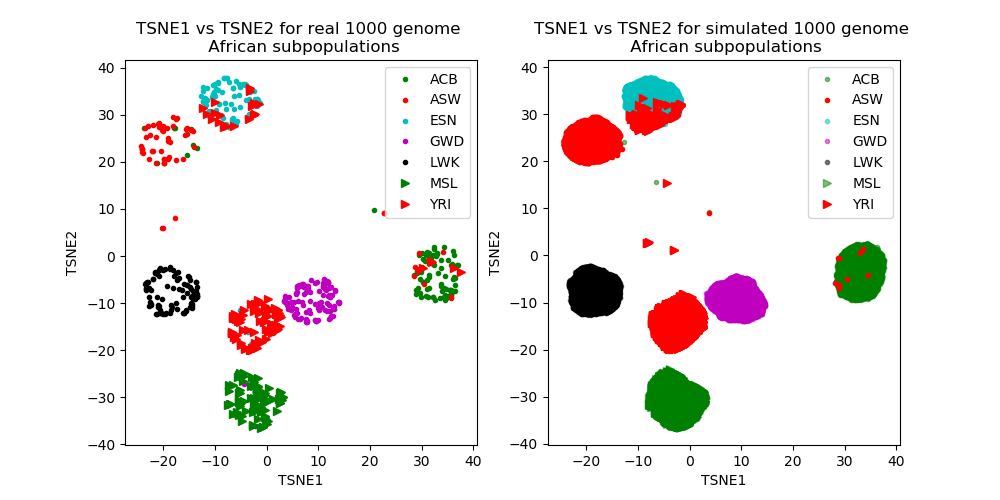
\includegraphics[scale = 0.65]{tsne.png}\\
\noindent Figure 1: Comparison of population whole genomes in 2 dimensional TSNE space.\\
\end{center}

\section{Differentiating attributes}

Many packages were built to simulate genetic data with different goals in mind. Genetic Architecture Model Emulator for Testing and Evaluating Software (GAMETEs) simulates simple and epistatic SNV/phenotype associations quickly but ignores LD patterns \cite{source:6}. Genome Simulation of Linkage and Association (GenomeSIMLA) uses forward time simulation to produce broadly realistic LD patterns. However, these patterns do not exactly match those of a particular dataset \cite{source:7}. Triadsim \cite{source:1} replicates exact LD patterns, but it requires (mother, father, kin) trios and takes an average CPU-time of 6.8 hours and an average peak RAM of 54.6 GB to simulate 10000 trios (20000 unrelated GWAS samples) with 4 breakpoints. REGENS uses the same recombination principles that Triadsim relies on, but it is 88.5 times faster (95\% CI (75.1, 105.0) via bootstrapping) and requires 6.2 times lower peak RAM (95\% CI (6.04, 6.33) via bootstrapping) on average over 10 replicate simulations (Intel(R) Xeon(R) CPU E5-2690 v4 2.60GHz processor). REGENS also recombines individuals instead of trios to simulate GWAS data with small publicly available genomic datasets, such as those in the 1000 Genomes project. This fact allows REGENS to accurately simulate the full genetic diversity of the world's population (representative figures are at \url{https://github.com/EpistasisLab/REGENS}). Finally, REGENS can simulate continuous and binary phenotypes that depend on any linear combination of products of f(SNV) values, where f transforms the standard SNP values of $\{0,1,2\}$ to represent nonlinear monoallelic effects (such as dominance). Example implementations of these features are in REGENS' GitHub repository.\\

\section{Inspiration and dependencies}

REGENS was inspired by Triadsim's idea to draw simulated breakpoints at locations with higher recombination rates, as well as well as by GAMETE's objective of simulating data quickly. REGENS relies on bed-reader, a spinoff of PySnpTools's core .bed file code \cite{source:8}, to optimally read uniformly re-sampled rows from plink bed files as 8 bit integers and then write the 8 bit integer simulated autosomal genotypes into new bed files. REGENS also relies on the 1000 genomes project's whole genomes from 26 distinct sub-populations \cite{source:9}, and it relies on those populations' corresponding genome-wide sex-averaged recombination rates inferred by the pyrho algorithm \cite{source:10}.\\  

\section*{Acknowledgements}

We acknowledge contributions from Carl Kadie, who developed PySnpTools, for implementing its ability to read and write plink bed files as 8 bit integers. This work was supported by NIH grant LM010098. 

\end{singlespace}

\bibliographystyle{unsrt}
\bibliography{paper}
\end{document}
